De manier waarop bestanden en mappen zijn ingedeeld op een disk noemen we een directory-tree\index{directory-tree}. De tree begint bij de root. De root directory\texttt{root directory} is de directory die direct na de C: komt en wordt weergegeven door een enkele \textbackslash. We kunnen snel daar de root-directory gaan met:
\begin{lstlisting}[style=DOS]
cd \
\end{lstlisting}
We staan nu aan het begin van de directory boom van de C-schijf. Met \texttt{dir} kunnen we zien welke directories er de eerste takken van de boom vormen:

\begin{minipage}[t]{\linewidth}
\raggedright
\adjustbox{valign=t}{%
	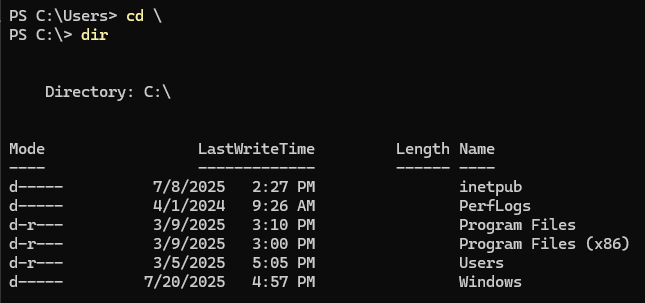
\includegraphics[width=0.99\linewidth]{Windows-rootdirs.png}%
}
\end{minipage}
